\documentclass[../differential_topology.tex]{subfiles}
\begin{document}
\section{Aula 06 - 03 de Setembro, 2026}
\subsection{Motivações}
\begin{itemize}
	\item Transversalidade
\end{itemize}
\subsection{Dimensão, Codimensão e Transversalidade}
Seja Z uma subvariedade de N de codimensão \(\ell \) em N; então, Z é localmente definida pela \textit{imagem inversa de um valor regular} de uma aplicação \(g:U\subseteq N\rightarrow \mathbb{R}^{\ell }\), onde U é um aberto de N, tal que M
\[
	V_{0} = Z\cap V = g^{-1}(0),
\]
correspondendo à parte de 0 ser um valor regular de g. Ademais, \(\varphi^{-1}(V_{0})=U)0\) é subvariedade de \(\mathbb{R}^{m}\) com \(\mathrm{codim}(U_{0})=\ell \).

A construção dessa g parte de considerar \(g:V\rightarrow \mathbb{R}^{\ell }\) com coordenadas \(g=(g_1, \dotsc , g_{\ell})\), com \(g_{i}:V\rightarrow \mathbb{R}\) para cada i.
Para que g seja submersão, é equivalente pedir que \(\{g_1(x), \dotsc , g_{\ell }(x)\}\) seja linearmente independente para todo x em V.

Podemos, então, provar o teorema enunciado na aula anterior:
\begin{theorem*}
	Sejam \(f:M\rightarrow N\) uma função suave e Z uma subvariedade de N; se f for transversal a Z, então \(f^{-1}(Z)\) é subvariedade de M e vale a relação
	\[
		\mathrm{codim}_{M}(f^{-1}(Z)) = \mathrm{codim}_{N}(Z).
	\]
\end{theorem*}
\begin{proof*}
	Seja p um ponto de M com \(f(p)\in Z\) e \(g:V\subseteq N\rightarrow \mathbb{R}^{\ell }\) tal que 0 é um valor regular de g e que \(V\cap Z = g^{-1}(0)\), onde V é um aberto em N contendo \(f(p)\).

	Observe que \(\mathrm{codim}(Z) = \ell \), pelas observações acima, e seja p um ponto do aberto U de M que satisfaça \(f(U)\subseteq V\); temos, então,
	\[
		f^{-1}(Z)\cap U = (g\circ f)^{-1}(0),
	\]

	\textbf{\underline{Afirmação}:} 0 é um valor regular de \((g\circ f):U\subseteq M\rightarrow \mathbb{R}^{\ell }\). Com efeito,
	\[
		(g\circ f)'(p) = g'(f(p))\cdot f'(p):T_{p}M\rightarrow \mathbb{R}^{\ell }.
	\]
	O fato de f ser transversal a Z equivale à relação
	\[
		T_{f(p)}N = f'(p)\cdot T_{p}M + T_{f(p)}Z,
	\]
	e, por isso,
	\[
		\underbrace{g'(f(p))\cdot T_{f(p)}N}_{\mathclap{\mathbb{R}^{n}}}=g'(f(p))\cdot f'(p)T_{p}M+\underbrace{g'(f(p))\cdot T_{f(p)}Z}_{\mathclap{0}}
	\]
	\begin{figure}[H]
		\begin{center}
			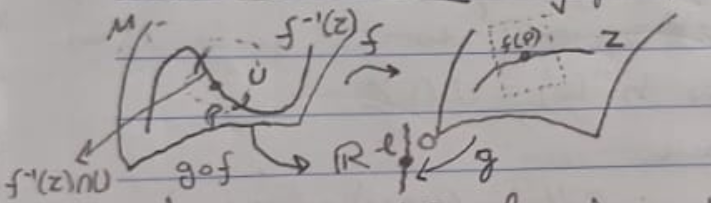
\includegraphics[height=0.6\textheight, width=0.6\textwidth, keepaspectratio]{./Images/06_transversal.png}
		\end{center}
	\end{figure}
	Portanto, \(g\circ f\) é sobrejetor e finalizamos a prova. \qedsymbol
\end{proof*}
\begin{tcolorbox}[
		skin=enhanced,
		title=Observação,
		fonttitle=\bfseries,
		colframe=black,
		colbacktitle=cyan!75!white,
		colback=cyan!15,
		colbacklower=black,
		coltitle=black,
		drop fuzzy shadow,
		%drop large lifted shadow
	]
	Quando temos duas variedades suaves M e N, uma subvariedade Z de N e um difeomorfismo \(f:M\rightarrow N\), podemos definir uma definição equivalente por
	\[
		f \pitchfork Z \Longleftrightarrow g\circ f :U\subseteq M\rightarrow \mathbb{R}^{\ell }
	\]
	for uma submersão para toda submersão \(g:V\rightarrow \mathbb{R}^{\ell }\) tal que \(g^{-1}(0)=Z\cap V\) com \(f(U)\subseteq V\).
\end{tcolorbox}
\begin{def*}
	Sejam M e Z subvariedades de N; diremos que \textbf{M e Z são transversais, \(\mathbf{M\pitchfork Z}\)}, se \(i\pitchfork Z\), onde i é a inclusão de M em N; em outras palavras, se
	\[
		T_{p}N = T_{p}M + T_{p}Z, \quad \forall p\in M\cap Z. \; \square
	\]
\end{def*}
Pode-se pensar na transversalidade entre subvariedades como se os espaços tangentes completassem o espaço todo da ``supervariedade'' delas, N.

\begin{theorem*}
	Sejam M, Z subvariedades de N. Se elas forem transversais, então \(M\cap Z\) é subvariedade de N tal que
	\[
		\mathrm{codim}(M\cap Z) = \mathrm{codim}(M)+\mathrm{codim}(Z).
	\]
\end{theorem*}
\begin{proof*}
	Denote a codimensão de M por k e a de Z por \(\ell \), e seja p um ponto da interseção dos dois.

	Como M é subvariedade de N, existe \(g:U\rightarrow \mathbb{R}^{k}\) com 0 valor regular e tal que \(g^{-1}(0)=U\cap M\), sendo U um aberto de N que contém p; similarmente, como Z é subvariedade de N, existe um mapa \(h:V\rightarrow \mathbb{R}^{\ell }\) com 0 como um valor regular e tal que \(h^{-1}(0) = V\cap Z\)

	Defina o difeomorfismo
	\begin{align*}
		G: & U\cap V\rightarrow\mathbb{R}^{k+\ell } \\
		   & x\longmapsto (g(x), h(x)),
	\end{align*}
	de forma que \(G^{-1}(0)=(U\cap V)\cap (M\cap Z)\) e 0 é valor regular de G. Por definição, para todo p em \(M\cap Z\),
	\[
		M\pitchfork Z \Longleftrightarrow T_{p}N = T_{p}M \cdot T_{p}Z = \mathrm{ker}(g'(p))+\mathrm{ker}(h'(p)),
	\]
	onde \(g=(g_1, \dotsc , g_{k}),\; h=(h_1, \dotsc , h_{\ell})\) com \(g_1'(p), \dotsc , g_{k}'(p)\) LI e \(h_{1}'(p), \dotsc , h_{\ell}'(p)\) também LI. Logo, \(\{g_{1}'(p), \dotsc , g_{k}'(p), h_{1}'(p), \dotsc , h_{\ell }'(p)\}\) são linearmente independentes, e portanto G é submersão. \qedsymbol

\end{proof*}

\end{document}
